% This file was created (at least in part) by the script ParseMdtoLatex by Louis du Plessis
% (Available from https://github.com/taming-the-beast)

\documentclass[11pt]{article}
%%%%%%%%%%%%%%%%%%%%%%%%%%%%%%%%%%%%%%%%%%%%%%%%%%%%%%%%%%%%%%%
% DO NOT EDIT THIS FILE UNLESS YOU KNOW WHAT YOU ARE DOING!!! %
%%%%%%%%%%%%%%%%%%%%%%%%%%%%%%%%%%%%%%%%%%%%%%%%%%%%%%%%%%%%%%%

% Useful packages
\usepackage[]{authblk}
\usepackage{graphicx}
\usepackage{color}
\usepackage{longtable}
\usepackage{hanging}
\usepackage{indentfirst}
\usepackage{setspace}
\usepackage{enumitem}
\usepackage{verbatim}
\usepackage{upgreek}
\usepackage{framed}
\usepackage{textcomp}
\usepackage{url}
\usepackage{soul}
\usepackage{amsmath,amsfonts,amssymb,mathrsfs}
\usepackage{fancyhdr}
\usepackage[compact]{titlesec}
\usepackage[T1]{fontenc}
\usepackage{lmodern}
\usepackage[utf8]{inputenc}
\usepackage[]{listings}
%\usepackage{fontspec}
\usepackage{placeins}
\usepackage{epstopdf}
\usepackage[export]{adjustbox}
\usepackage{tikz}
\usepackage[breaklinks]{hyperref}
\usepackage[all]{hypcap}


% References
\usepackage[backend=bibtex,hyperref=true,citestyle=authoryear,bibstyle=authortitle,firstinits=true,terseinits=true,doi=false,url=false,eprint=false,maxbibnames=10,maxcitenames=2]{biblatex}
\DeclareCiteCommand{\cite}
  {\usebibmacro{prenote}}
  {\usebibmacro{citeindex}%
   \printtext[bibhyperref]{\usebibmacro{cite}}}
  {\multicitedelim}
  {\usebibmacro{postnote}}

\DeclareCiteCommand*{\cite}
  {\usebibmacro{prenote}}
  {\usebibmacro{citeindex}%
   \printtext[bibhyperref]{\usebibmacro{citeyear}}}
  {\multicitedelim}
  {\usebibmacro{postnote}}

\DeclareCiteCommand{\parencite}[\mkbibparens]
  {\usebibmacro{prenote}}
  {\usebibmacro{citeindex}%
    \printtext[bibhyperref]{\usebibmacro{cite}}}
  {\multicitedelim}
  {\usebibmacro{postnote}}

\DeclareCiteCommand*{\parencite}[\mkbibparens]
  {\usebibmacro{prenote}}
  {\usebibmacro{citeindex}%
    \printtext[bibhyperref]{\usebibmacro{citeyear}}}
  {\multicitedelim}
  {\usebibmacro{postnote}}

\DeclareCiteCommand{\footcite}[\mkbibfootnote]
  {\usebibmacro{prenote}}
  {\usebibmacro{citeindex}%
  \printtext[bibhyperref]{ \usebibmacro{cite}}}
  {\multicitedelim}
  {\usebibmacro{postnote}}

\DeclareCiteCommand{\footcitetext}[\mkbibfootnotetext]
  {\usebibmacro{prenote}}
  {\usebibmacro{citeindex}%
   \printtext[bibhyperref]{\usebibmacro{cite}}}
  {\multicitedelim}
  {\usebibmacro{postnote}}

\DeclareCiteCommand{\textcite}
  {\boolfalse{cbx:parens}}
  {\usebibmacro{citeindex}%
   \printtext[bibhyperref]{\usebibmacro{textcite}}}
  {\ifbool{cbx:parens}
     {\bibcloseparen\global\boolfalse{cbx:parens}}
     {}%
   \multicitedelim}
  {\usebibmacro{textcite:postnote}}

\newcommand{\citep}{\parencite}
\newcommand{\citet}{\textcite}
\defbibheading{relevref}[\refname]{\section*{Relevant References}}

\renewcommand{\postnotedelim}{\iffieldpages{postnote}{\addcolon}{\addcomma\space}} 
\DeclareFieldFormat{postnote}{#1} 

\DeclareFieldFormat[article, inbook, incollection, inproceedings, patent, thesis, unpublished]{title}{#1}
\DeclareFieldFormat[article, inbook, incollection, inproceedings, patent, thesis, unpublished]{journaltitle}{\mkbibemph{#1}\nopunct}
\DeclareFieldFormat[article, inbook, incollection, inproceedings, patent, thesis, unpublished]{volume}{{#1}\addcolon} %puts volume number in parens
%\DeclareFieldFormat[article, inbook, incollection, inproceedings, patent, thesis, unpublished]{year}{\mkbibparens{#1}\nopunct} %puts year in parens

\DeclareFieldFormat[article, incollection, patent, thesis, unpublished]{pages}{{\nopp#1}}

\DeclareFieldFormat{sentencecase}{\MakeSentenceCase{#1}}

\renewbibmacro*{title}{%
  \ifthenelse{\iffieldundef{title}\AND\iffieldundef{subtitle}}
    {}
    {\ifthenelse{\ifentrytype{article}\OR\ifentrytype{inbook}%
      \OR\ifentrytype{incollection}\OR\ifentrytype{inproceedings}%
      \OR\ifentrytype{inreference}}
      {\printtext[title]{%
        \printfield[sentencecase]{title}%
        \setunit{\subtitlepunct}%
        \printfield[sentencecase]{subtitle}}}%
      {\printtext[title]{%
        \printfield[titlecase]{title}%
        \setunit{\subtitlepunct}%
        \printfield[titlecase]{subtitle}}}%
     \newunit}%
  \printfield{titleaddon}}

\DefineBibliographyStrings{english}{% various adjustments to common bib entry strings
urlseen = {Accessed:},% What goes in front of the date a URL was accessed/retrieved etc.
editor = {(Ed)},%Ed – no dot, in brackets
editors = {(Eds)},% Eds – no dot, in brackets
byeditor = {(Ed.)}}% ‘Edited by’ for edited works

\DeclareNameAlias{default}{last-first}

\renewbibmacro{in:}{}

\renewbibmacro{publisher+location+date}{
  \iflistundef{publisher}
    {}
    {\printlist{publisher}%
       {\addcomma\space}%
      \iflistundef{location}
        {}
        {\printlist{location}}%
    }
}

\DeclareBibliographyDriver{article}{%
\usebibmacro{bibindex}%
\usebibmacro{begentry}%
\usebibmacro{author/translator+others}%
\newunit\newblock
\printfield{year}%
\setunit{\labelnamepunct}\newblock
\usebibmacro{title}%
\newunit
\printlist{language}%
\newunit\newblock
\usebibmacro{byauthor}%
\newunit\newblock
\usebibmacro{bytranslator+others}%
\newunit\newblock
\printfield{version}%
\newunit\newblock
%\usebibmacro{in:}% %mit in:
\usebibmacro{journal}%
\newunit\newblock
\printfield{volume}%
\newunit\newblock
\usebibmacro{byeditor+others}%
\newunit\newblock
\usebibmacro{note+pages}%
\newunit\newblock
\iftoggle{bbx:isbn}
{}%
\newunit\newblock
\usebibmacro{doi+eprint+url}%
\newunit\newblock
\usebibmacro{addendum+pubstate}%
\newunit\newblock
\usebibmacro{pageref}%
\usebibmacro{finentry}}

\DeclareBibliographyDriver{inproceedings}{%
\usebibmacro{bibindex}%
\usebibmacro{begentry}%
\usebibmacro{author/translator+others}%
\newunit\newblock
\printfield{year}%
\setunit{\labelnamepunct}\newblock
\usebibmacro{title}%
\newunit
\printlist{language}%
\newunit\newblock
\usebibmacro{byauthor}%
\newunit\newblock
\usebibmacro{bytranslator+others}%
\newunit\newblock
\printfield{version}%
\newunit\newblock
%\usebibmacro{in:}% %mit in:
\usebibmacro{booktitle}%
\newunit\newblock
\printfield{volume}%
\newunit\newblock
\usebibmacro{byeditor+others}%
\newunit\newblock
\usebibmacro{publisher+location+date}%
\newunit\newblock
\usebibmacro{note+pages}%
\newunit\newblock
\usebibmacro{pageref}%
\usebibmacro{finentry}}

\DeclareBibliographyDriver{book}{%
\usebibmacro{bibindex}%
\usebibmacro{begentry}%
\usebibmacro{author/translator+others}%
\newunit\newblock
\printfield{year}%
\setunit{\labelnamepunct}\newblock
\usebibmacro{title}%
\newunit
\printlist{language}%
\newunit\newblock
\usebibmacro{byauthor}%
\newunit\newblock
\usebibmacro{bytranslator+others}%
\newunit\newblock
%\usebibmacro{in:}% %mit in:
\usebibmacro{booktitle}%
\newunit\newblock
\printfield{volume}%
\newunit\newblock
\usebibmacro{publisher+location+date}%
\newunit\newblock
\usebibmacro{note+pages}%
\newunit\newblock
\usebibmacro{pageref}%
\usebibmacro{finentry}}

% Page margins
\setlength{\evensidemargin}{0in}
\setlength{\headheight}{0in}
\setlength{\headsep}{0in}
\setlength{\oddsidemargin}{-0.25in}
\setlength{\paperheight}{11in}
\setlength{\paperwidth}{8.5in}
\setlength{\tabcolsep}{0in}
\setlength{\textheight}{9in}
\setlength{\textwidth}{7in}
\setlength{\topmargin}{0in}
\setlength{\topskip}{0in}
\setlength{\voffset}{0in}
\parskip = 0.15in
\pagestyle{plain}
\setlength{\parindent}{0cm}

% No white space between list items
\setlist{nolistsep}

% Hyperlink setup
\hypersetup{colorlinks=true,linkcolor=linkscol,citecolor=citescol,urlcolor=urlscol}

% Settings for code blocks
\lstset{backgroundcolor=\color[rgb]{0.972,0.972,0.972},
    tabsize=4,
    rulecolor=,
        basicstyle=\scriptsize,
        upquote=true,
        aboveskip={1.5\baselineskip},
        columns=fixed,
        showstringspaces=false,
        extendedchars=true,
        breaklines=true,
        prebreak = \raisebox{0ex}[0ex][0ex]{\ensuremath{\hookleftarrow}},
        frame=single,
        showtabs=false,
        showspaces=false,
        showstringspaces=false,
        identifierstyle=\ttfamily,
        keywordstyle=\color[rgb]{0,0,1},
        commentstyle=\color[rgb]{0.133,0.545,0.133},
        stringstyle=\color[rgb]{0.627,0.126,0.941}
}

% Colour definitions
\definecolor{citescol}{RGB}{194,101,1}
\definecolor{urlscol}{RGB}{0,150,206}
\definecolor{linkscol}{RGB}{149,0,207}
\definecolor{mycol}{RGB}{25,23,191}
\definecolor{outputcol}{RGB}{34,139,34}
\definecolor{tcol}{RGB}{165,0,14}







% TODO: The rest of the file needs to be cleaned up!
%       Past this point I am not sure what is necessary or not - Louis


\DeclareMathAlphabet{\msfsl}{T1}{cmr}{m}{it}
\DeclareMathAlphabet{\msyf}{OMX}{pcr}{m}{it}
\newcommand{\alf}{\upalpha}
\newcommand{\hilight}[1]{\colorbox{yellow}{#1}}

\newcommand{\levelone}[1]{
\bigskip
\noindent{\LARGE{\textsc{#1}}}
\vspace {0.05in}
}

\newcommand{\leveltwo}[1]{
\bigskip
\noindent{\Large{\textit{#1}}}
\vspace {-1mm}
}

\newcommand{\descriptionhead}[1]{
\noindent{\textcolor{mycol}{\textbf{\textit{#1}}}}\\ \vspace{-7mm}
}

\newcommand{\dhead}[1]{
\noindent{\textbf{\textit{#1 --}}}
}

\newcommand{\exs}[1]{
\vspace{-4mm}
\begin{itemize}
\item #1 \\ \vspace{-8mm}
\end{itemize}
}


\newcommand{\nbo}[1]{{\color{red}{#1}}}


\newcommand{\stepbullet}{\noindent \textbullet \ }
\newcommand{\mi}[1]{\textbf{\textit{#1}}}


\newcommand{\levelthree}[1]{\textit{#1 --}}


%\bibliographystyle{apalike}
%\bibpunct[; ]{(}{)}{;}{a}{,}{;}


\usepackage[breaklinks]{hyperref}
\usepackage[all]{hypcap}
\hypersetup{colorlinks=true,linkcolor=linkscol,citecolor=citescol,urlcolor=urlscol}

% Some macros for software packages
\newcommand{\R}{\texttt{R} }
\newcommand{\TESS}{\texttt{TESS}}
\newcommand{\PBD}{\texttt{PBD}}
\newcommand{\DDD}{\texttt{DDD}}
\newcommand{\Laser}{\texttt{laser}}
\newcommand{\TreePar}{\texttt{TreePar}}
\newcommand{\diversitree}{\texttt{diversitree}}
\newcommand{\RevBayes}{\texttt{RevBayes}}
\newcommand{\Rev}{\texttt{Rev}}
\newcommand{\MrBayes}{\texttt{MrBayes}}
\newcommand{\BEAST}{\texttt{BEAST}}
\newcommand{\PhyloBayes}{\texttt{PhyloBayes}}
\newcommand{\PAML}{\texttt{PAML}}

\let\otheriint\iint
\let\iint\relax
\usepackage{ wasysym }







\definecolor{shadecolor}{RGB}{194,225,255}

\setlength{\tabcolsep}{5pt}
\setlength{\topmargin}{-0.4in}
\setlength{\headheight}{14.5pt}
\pagestyle{fancy}

\newcommand{\taha}[1]{{\textcolor{red}{[TAH comment: #1]}}} % TAH comment

\titlespacing{\section}{0pt}{*0}{*0}
\titlespacing{\subsection}{0pt}{*0}{*0}
\titlespacing{\subsubsection}{0pt}{*0}{*0}

\titleformat{\section}
  {\normalfont\Large\bfseries\color{mycol}}
  {\thesection}{1em}{}

\titleformat{\subsection}
  {\normalfont\large\bfseries\color{mycol}}
  {\thesubsection}{1em}{}

\titleformat{\subsubsection}
  {\normalfont\bfseries\color{mycol}}
  {\thesubsubsection}{1em}{}

% command for MrBayes command-line step
\newcommand{\cl}[1]{{\texttt{\textbf{#1}}}}
\newcommand{\colx}[1]{{\textcolor{tcol}{#1}}}
\newcommand{\mbcl}[1]{\exs{\cl{MrBayes > {#1}}}}

\newcommand{\rbprmt}{RevBayes > } 
\newcommand{\rbcl}[1]{\exs{\cl{\rbprmt{#1}}}}
\newcommand{\rbout}[1]{\exs{\cl{\textcolor{outputcol}{#1}}}}
\newcommand{\rbdn}{{\Large \symbol{126}}} % This makes a copy/pasteable tilde
\newcommand{\rbclml}[1]{\exs{\cl{\ \ \ \ \ \ \ \ \ \ \ {#1}}}}

% text box settings
% requires compiling w/ XeLaTeX
%\newfontfamily\listingsfont[Scale=1.0]{Courier New}
%\lstset{basicstyle=\listingsfont, columns=texcl}
%\defaultfontfeatures{Mapping=tex-text}


\makeatletter
\lst@CCPutMacro\lst@ProcessOther {"2D}{\lst@ttfamily{-{}}{-{}}}
\@empty\z@\@empty
\makeatother



\setlength{\topmargin}{-0.4in}
\setlength{\headheight}{14.5pt}
\pagestyle{fancy}



\definecolor{lg}{gray}{0.75}
\def\gcirc{{%
    \setbox0\hbox{$\fullmoon$}%
    \rlap{\hbox to \wd0{\hss{$\textcolor{lg}{\newmoon}$}\hss}}\box0
}}

% Add your bibtex library here
\addbibresource{refs}


%%%%%%%%%%%%%%%%%%%%
% Do NOT edit this %
%%%%%%%%%%%%%%%%%%%%
\begin{document}
\renewcommand{\headrulewidth}{0.5pt}
\headsep = 20pt
\lhead{ }
\rhead{\textsc {BEAST v2 Tutorial}}
\thispagestyle{plain}


%%%%%%%%%%%%%%%%%%
% Tutorial title %
%%%%%%%%%%%%%%%%%%
\begin{center}

	% Enter the name of your tutorial here
	\textbf{\LARGE Tutorial using BEAST v2.5.2}\\\vspace{2mm}

	% Enter a short description of your tutorial here
	\textbf{\textcolor{mycol}{\Large Fast relaxed clock model}}\\

	\vspace{4mm}

	% Enter the names of all the authors here
	{\Large {\em Rong Zhang and Alexei Drummond}}
\end{center}

This tutorial introduces ConstantDistance operator to improve the efficiency of BEAST analysis under relaxed clock models. The proposal kernel in the presented operator changes evolutionary rates and divergence times at the same time, under the constraint that the implied genetic distances remain constant. Specifically, the proposal operates on the divergence time of an internal node and the three adjacent branch rates. For the root of a phylogenetic tree, there are three strategies included, named Simple Distance, Small Pulley and Big Pulley. The descriptions below will provide guidance step by step to estimate evolutionary rates and divergence times using BEAST2 software.

%%%%%%%%%%%%%%%%%
% Tutorial body %
%%%%%%%%%%%%%%%%%

\section{Introduction}\label{introduction}
Bayesian phylogenetic inference via MCMC is computationally intensive for large data sets. Two approaches to improve efficiency are (i) by making faster likelihood calculations, and (ii) by incorporating more effective proposal kernels. However, the overall efficiency of the sampling process also depends strongly on the construction of the proposal mechanism. An effective proposal mechanism is proficient at exploring the posterior distribution, and can do so with fewer steps in the MCMC chain. Therefore fewer likelihood calculations are required, since each step in the chain requires a likelihood calculation.

The operator presented in this tutorial, ConstantDistance operator, is based on an uncorrelated relaxed clock model, in which the rates vary from branch to branch, drawn independently and identically from a given prior distribution, such as the log-normal distribution (\cite{drummond2006relaxed}). As a result, the rates can vary markedly between parent and child branches.

More specifically, the presented operator searches within a subspace of constant genetic distances. Namely, the proposed operator changes both divergence times of nodes and neighbouring branch rates so that implied genetic distances are not changed. For time-reversible substitution models the phylogenetic likelihood will also be unchanged under this operation.

It is demonstrated that the proposed operator is able to improve the performance by giving better estimates and using less running time. Measured by effective samples per hour, the proposed operator is more than an order of magnitude faster than the current operators in BEAST2 on real and simulated data sets.

\section{Required programs}\label{programs}
\begin{itemize}
\item BEAST2 - Bayesian Evolutionary Analysis Sampling Trees

BEAST2 is a software platform for phylogenetic analysis based on Bayesian MCMC algorithms. This tutorial is written for BEAST v2.5.0 (\cite{bouckaert2014beast}).
\item BEAUti - Bayesian Evolutionary Analysis Utility

BEAUti is a graphical user interface tool to generate XML files that BEAST2 takes as input. It provides users with configuration options that are necessary for Bayesian phylogenetic analysis, such as prior distributions of parameter and various evolutionary models.

\end{itemize}

You may also need the following programs to analyse the output files of BEAST2.
\begin{itemize}
\item Tracer

This program analyses .log file which records the sampled states in Bayesian MCMC chain by BEAST2 (\url{http://tree.bio.ed.ac.uk/software/tracer}). It displays distributions of sampled parameters and calculates Effective Sample Size (ESS) automatically.
\item FigTree

This program reads .trees file and visualises trees sampled during MCMC chain (\url{http://tree.bio.ed.ac.uk/software/figtree}). The users can designate phylogenetic properties to show on the plotted trees, such as node ages, rates, branch length and so on.
\item TreeAnnotator

This program summaries trees in .tree file based on posterior distribution and gives a maximum clade credibility tree (\url{https://beast2.blogs.auckland.ac.nz/treeannotator/}). 
\end{itemize}

\section{Practical analysis}\label{analysis}
\subsection{Set up operator package}
Currently, the operator is developed as a package of BEAST2. Before the analysis, firstly download \href{https://github.com/Rong419/ConstantDistanceOperator.git}{ConstantDistance Operator} from Github repository and set up the dependency on BEAST2.

\subsection{Set up BEAUti}
\begin{enumerate}
\item Start BEAUti

After setting the main class as ``beast.app.beauti.Beauti" in configuration, you will see the interface of BEAUti, as is shown in Fig.\ref{fig:start-beauti}.
\begin{figure}
\centering
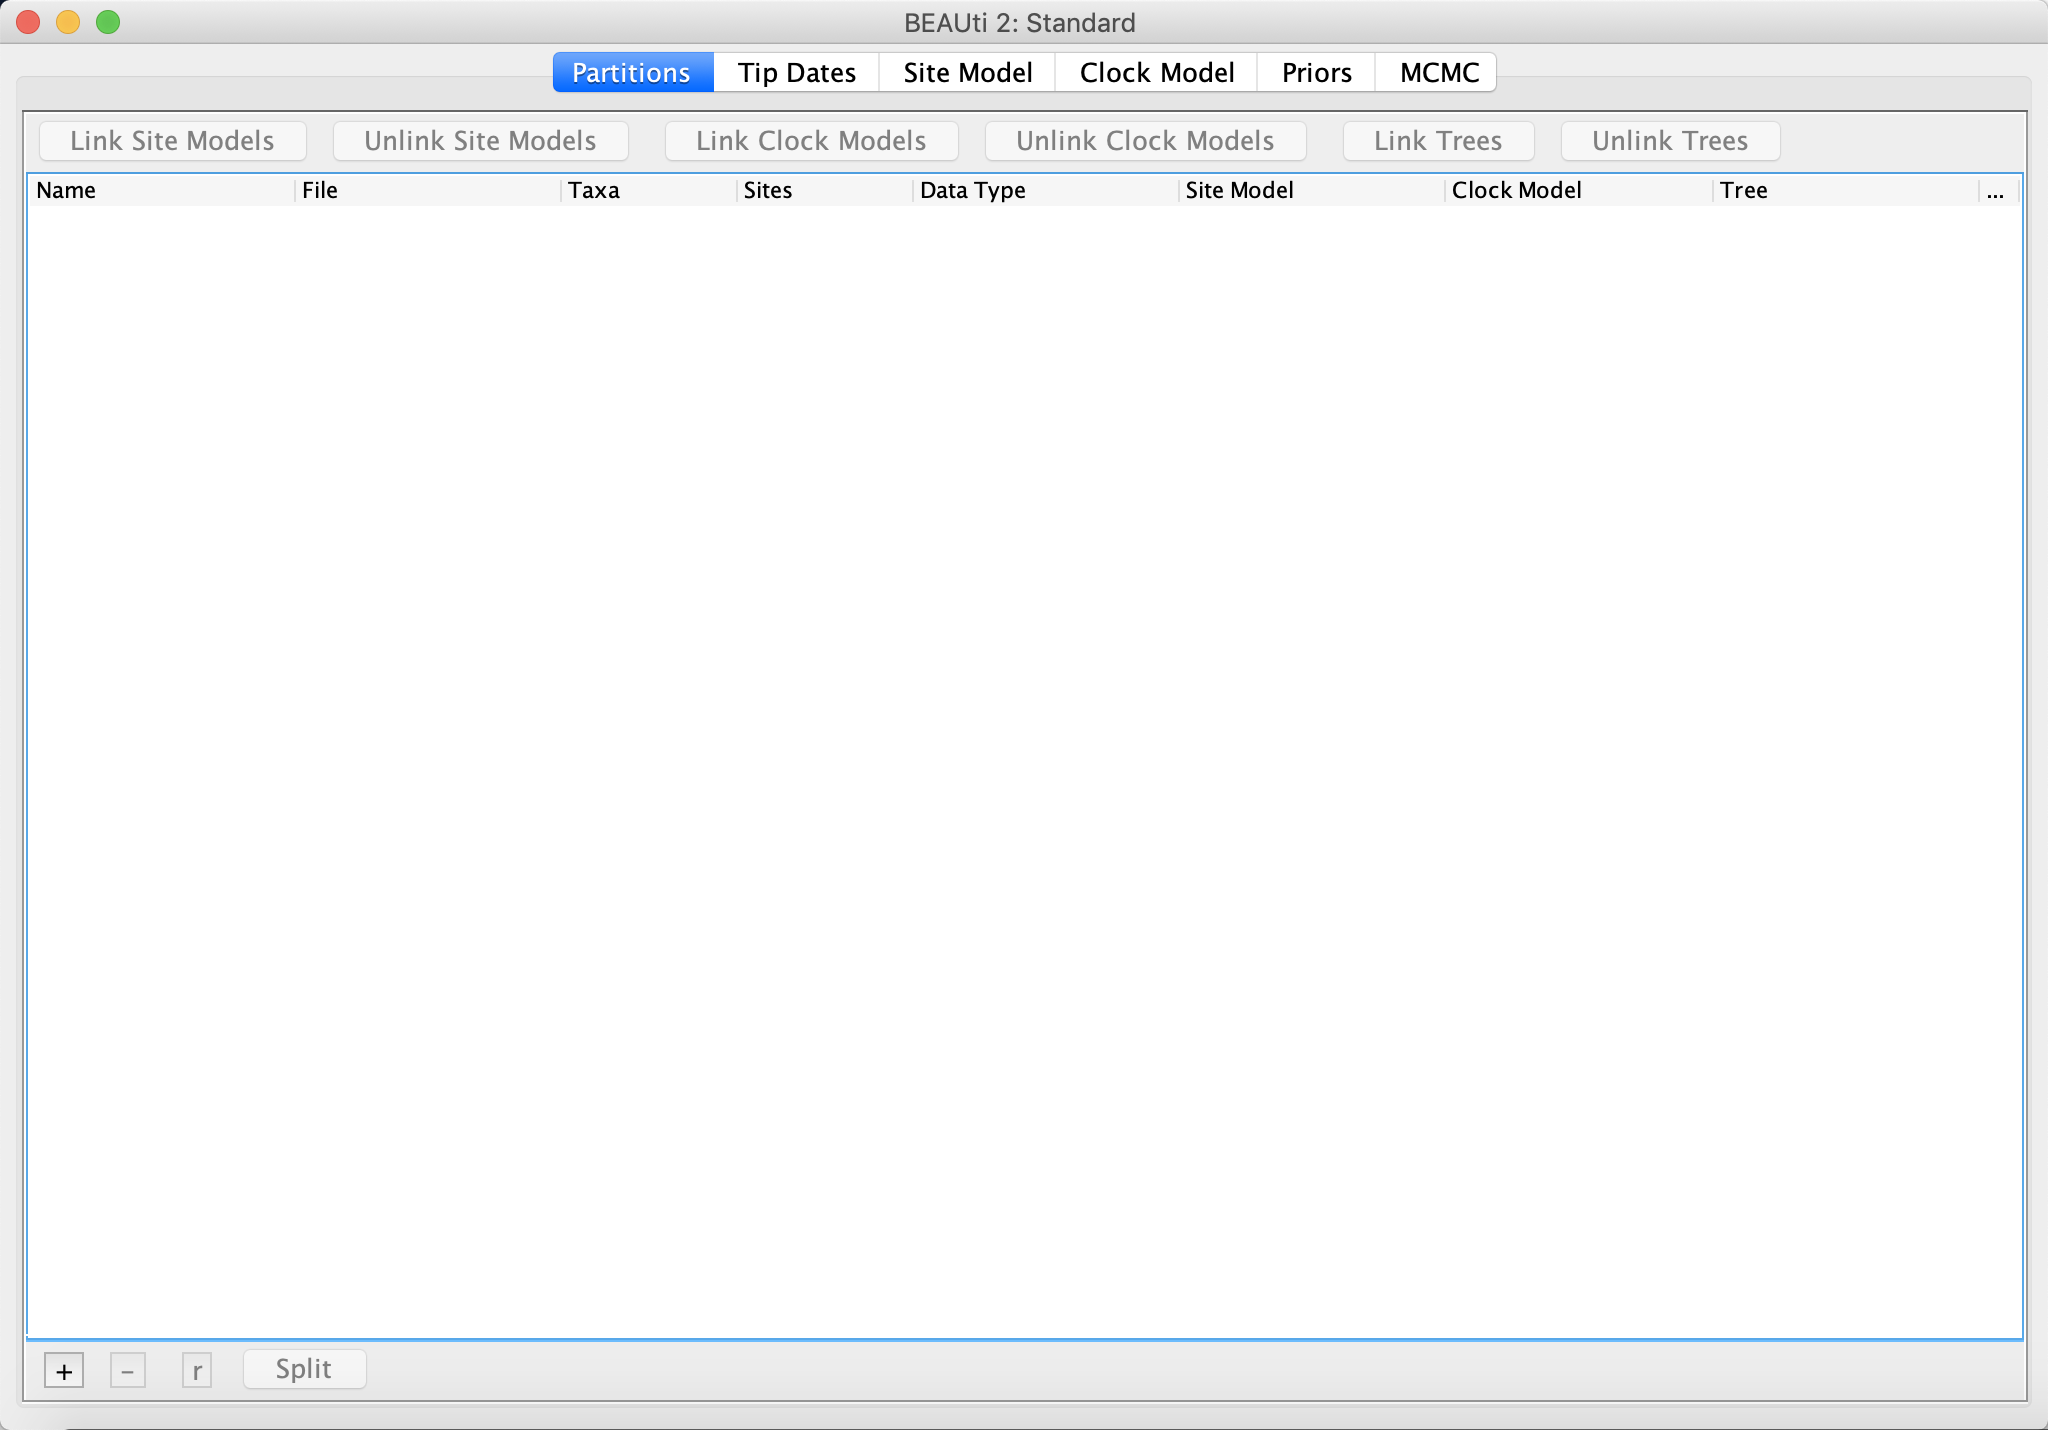
\includegraphics[width=0.750000\textwidth]{figures/beauti_start.png}
\caption{beati start}
 \label{fig:start-beauti}
\end{figure}

\item Import alignment
Click on ``File -> Import Alignment", and than choose the .nex data file. Here we import primates.nex as an example (Fig.\ref{fig:import-alignment}).
\begin{figure}
\centering
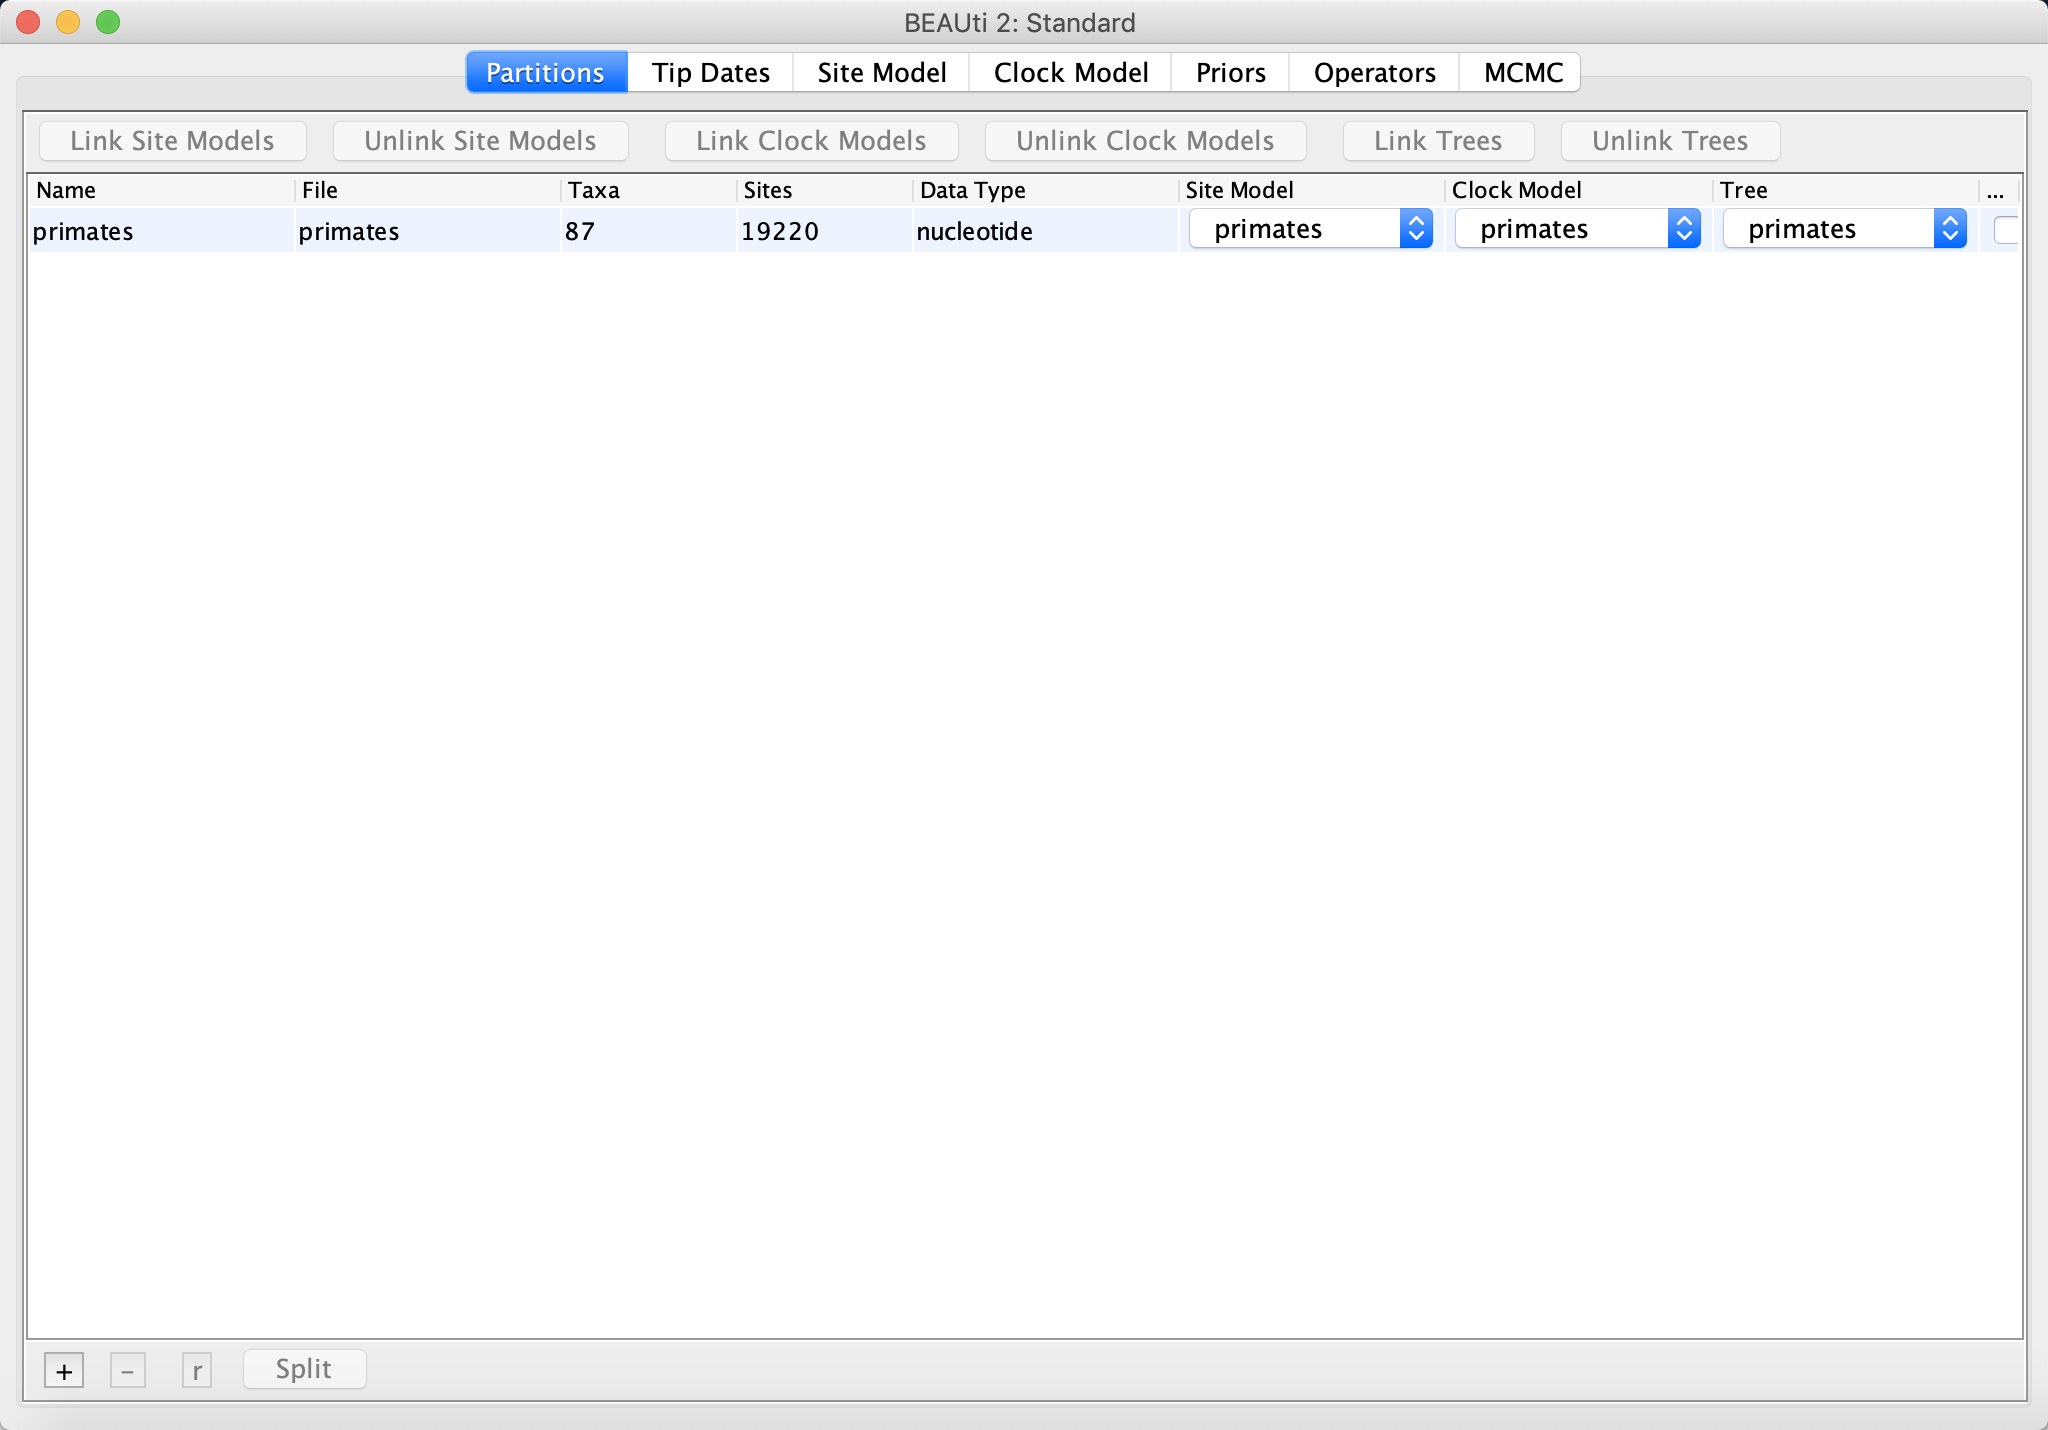
\includegraphics[width=0.750000\textwidth]{figures/import_alignment.png}
\caption{import alignment}
 \label{fig:import-alignment}
\end{figure}

\item Specify clock model

To use the operator, we assume an uncorrelated relaxed clock model. Specifically, as is illustrated in Fig.\ref{fig: clock model}, we need to click on "Clock Model" panel and then choose "Fast Relaxed Clock Log Normal" in the drop-down menu.
\begin{figure}
\centering
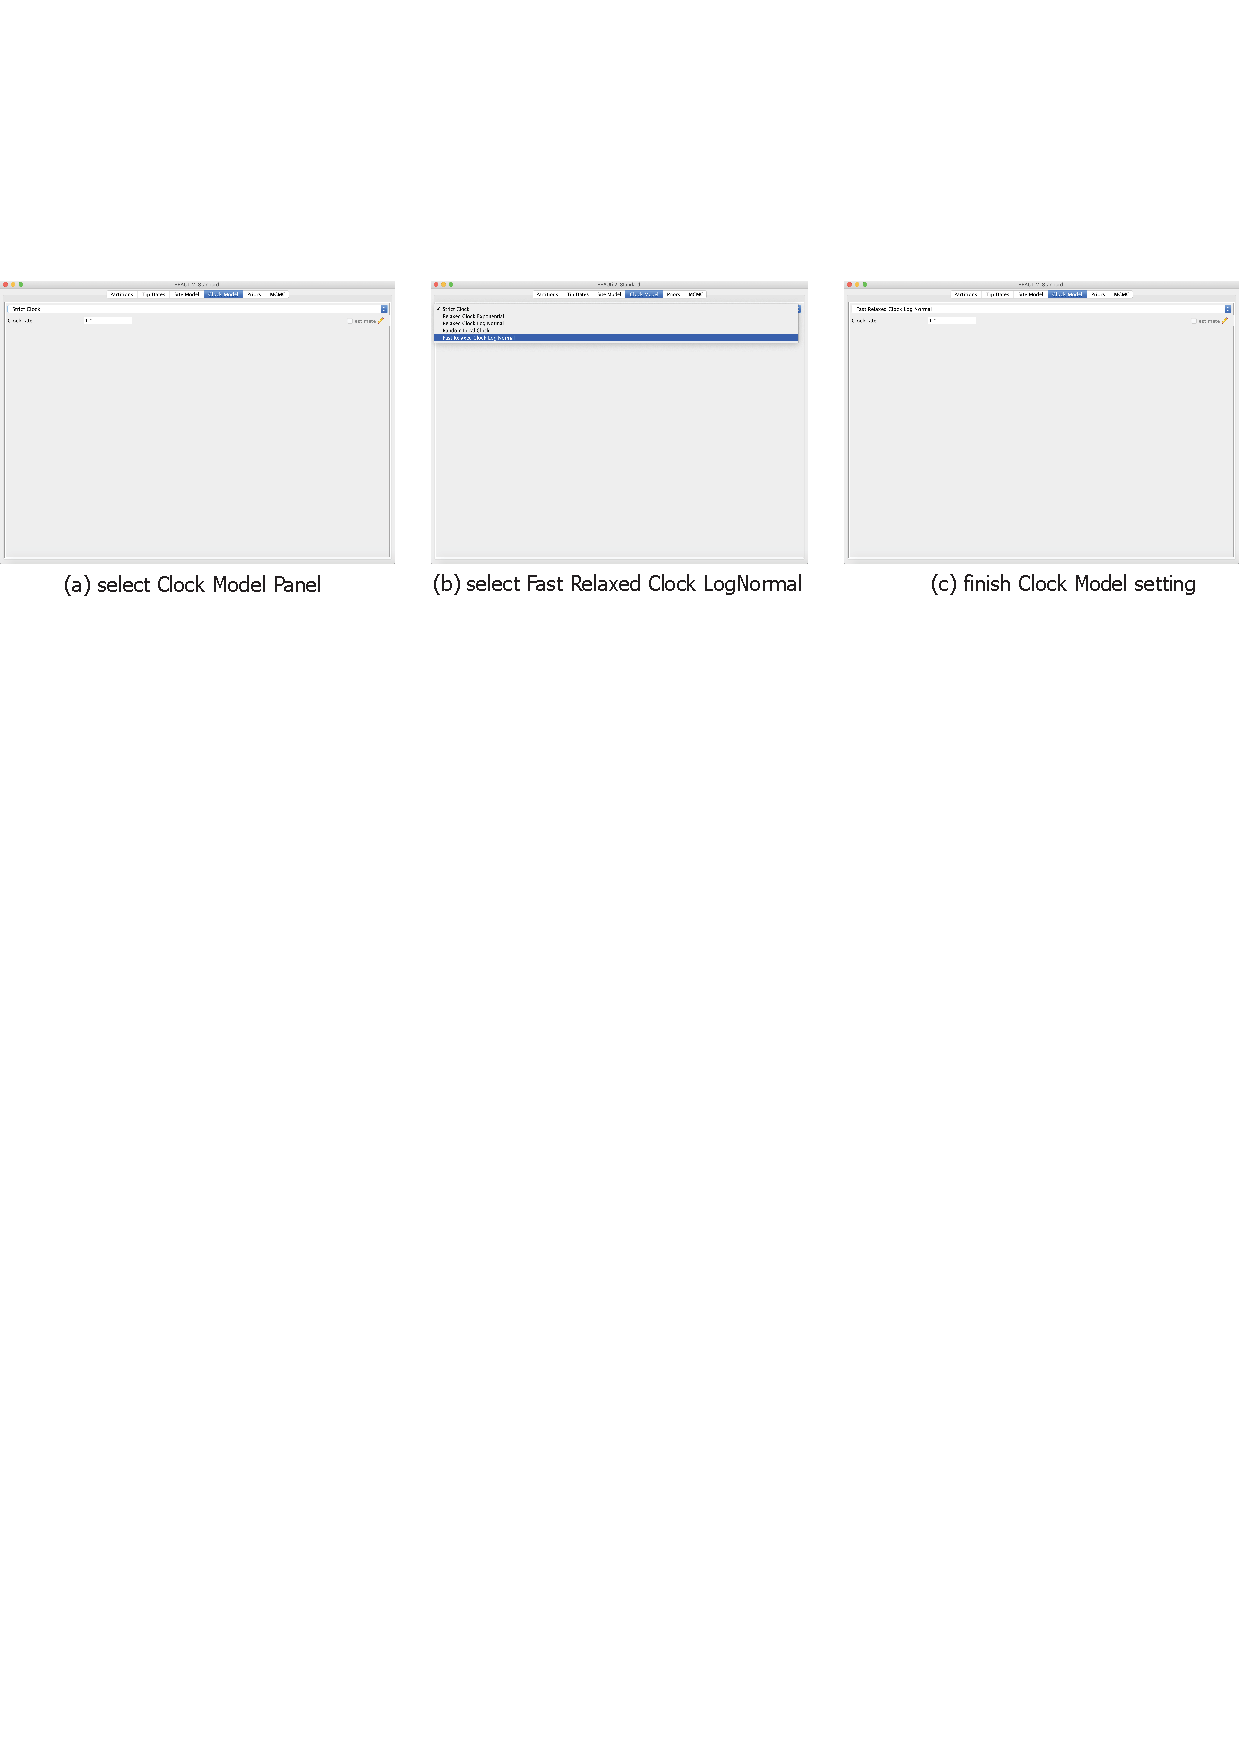
\includegraphics[width=0.750000\textwidth]{figures/clockmodel.pdf}
\caption{specify clock model}
 \label{fig: clock model}
\end{figure}

\item Specify priors

Under the selected clock model, the mandatory prior distribution includes prior on evolutionary rates (Log Normal distribution) and hyper prior on the standard deviation of the Log Normal distribution, as is shown in the red rectangles in Fig.\ref{fig: prior}. It should be pointed out that the mean of rate values are fixed to one, which is consistent with the clock rate.
\begin{figure}
\centering
\includegraphics[width=0.750000\textwidth]{figures/prior.pdf}
\caption{specify prior}
 \label{fig: prior}
\end{figure}

\item Specify operators
In the operators panel (click on "View" -> "Show Operators panel"), the ConstantDistance operator includes one operator on internal nodes and three operators on root, as can be seen in the red rectangle in Fig.\ref{fig: operator-panel}. Based on different data sets, you are able to specify different weights on the corresponding operators, instead of using default configuration.  
\begin{figure}
\centering
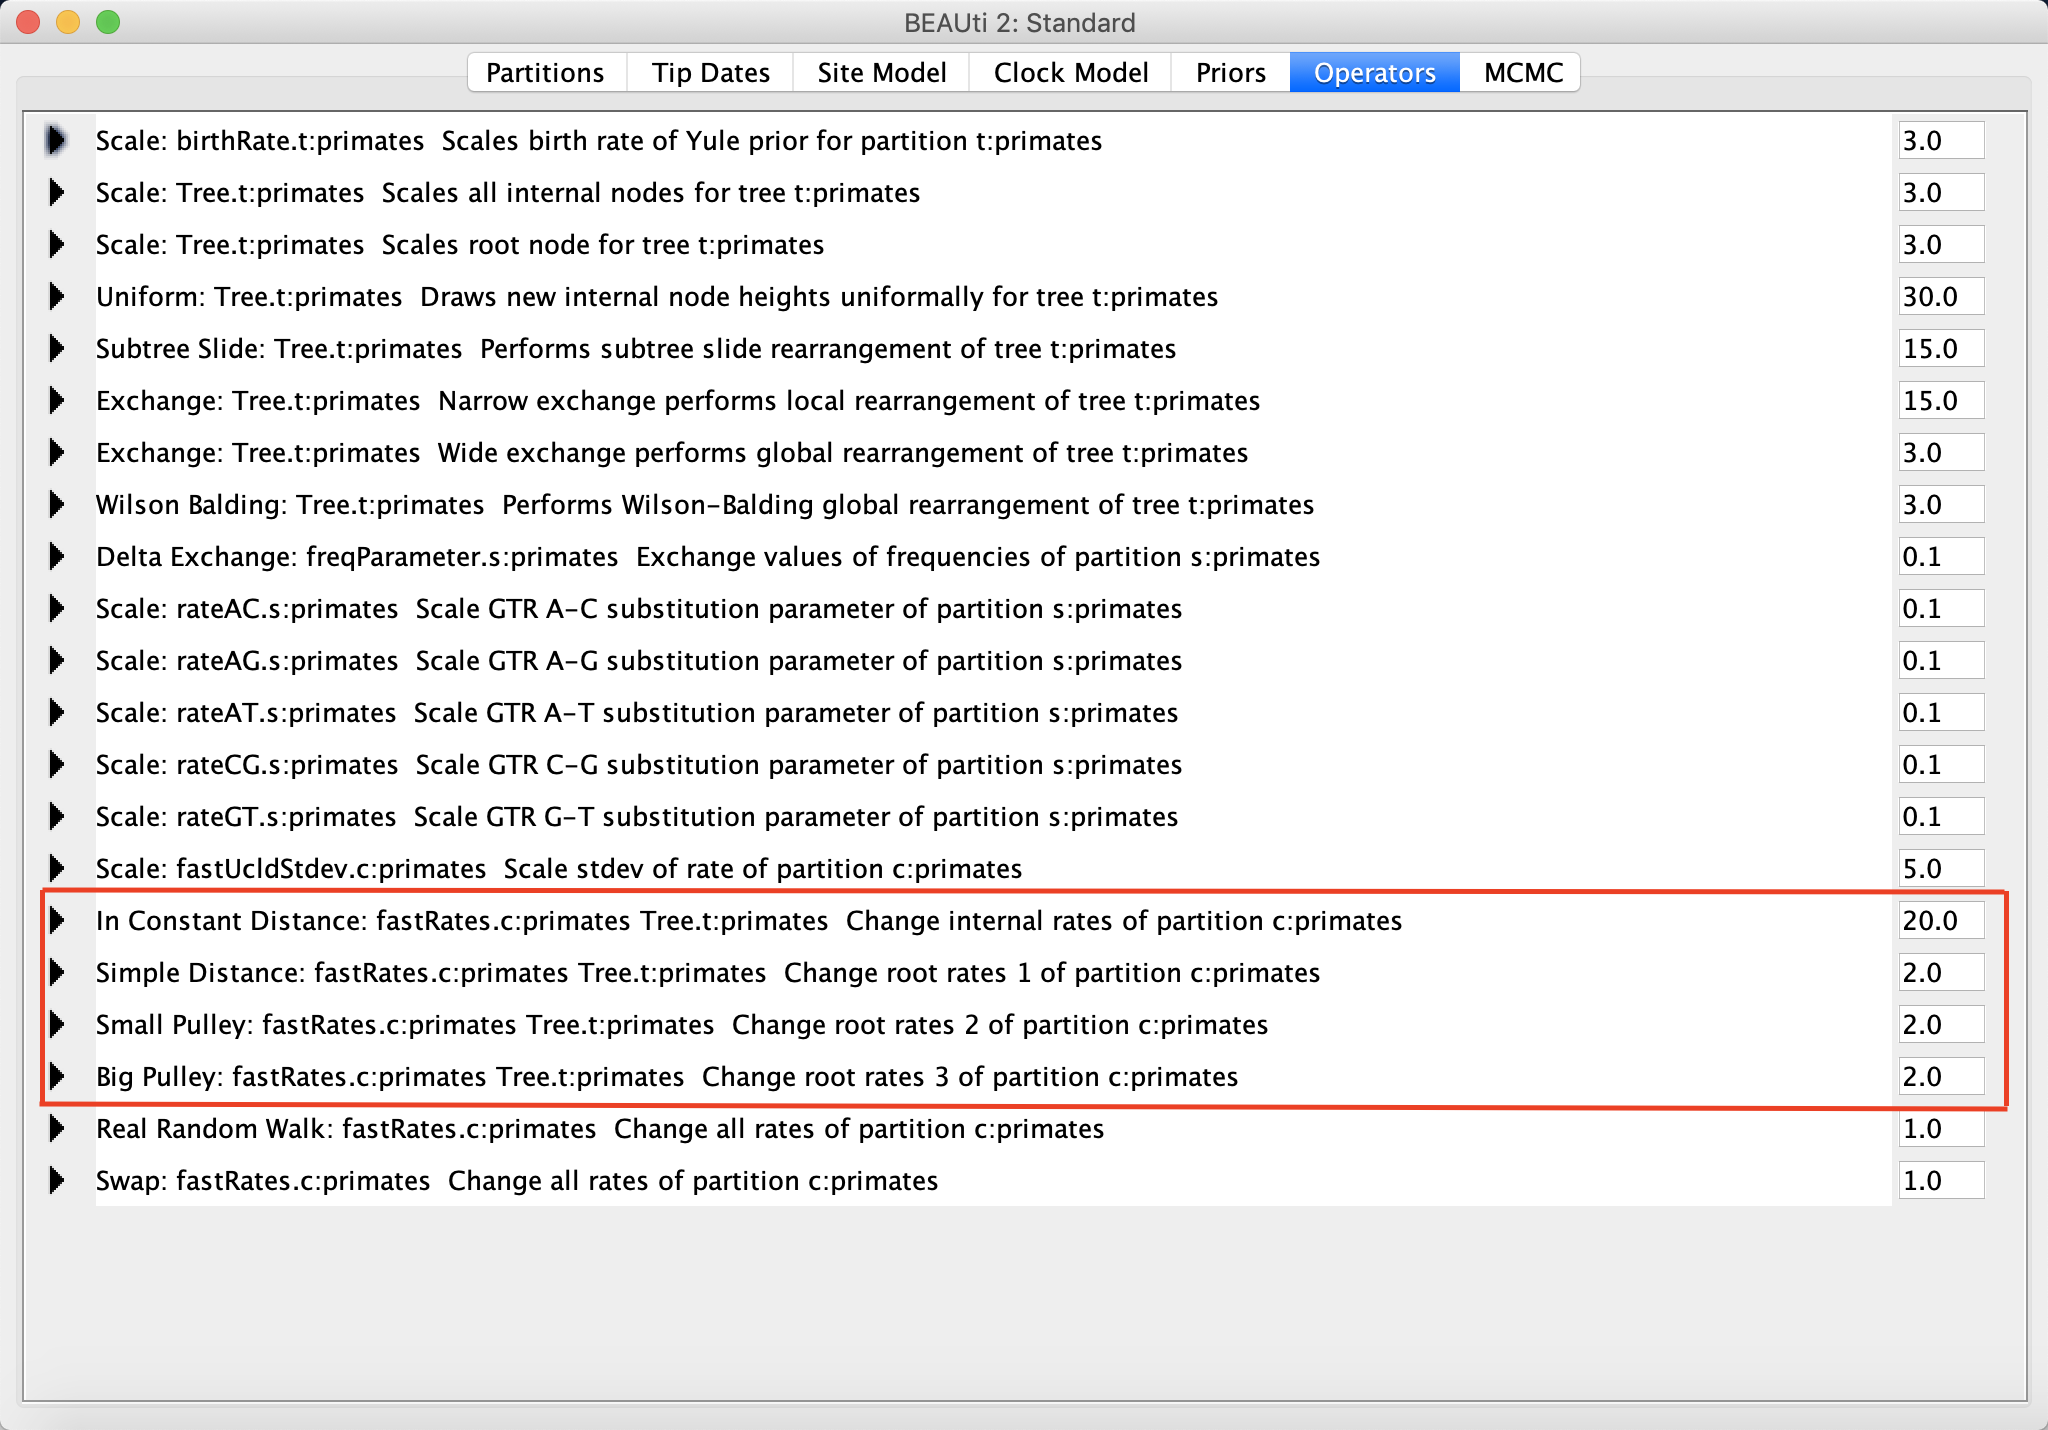
\includegraphics[width=0.750000\textwidth]{figures/operator_panel.png}
\caption{specify operator}
 \label{fig: operator-panel}
\end{figure}

\item Set up MCMC chain

As is shown in Fig.\ref{fig: trace-log}, you are able to confirm that the rates and standard deviations will be correctly logged in .log file. For different analysis requirements, you are also able to make modifications by click on ``edit" botton.
\begin{figure}
\centering
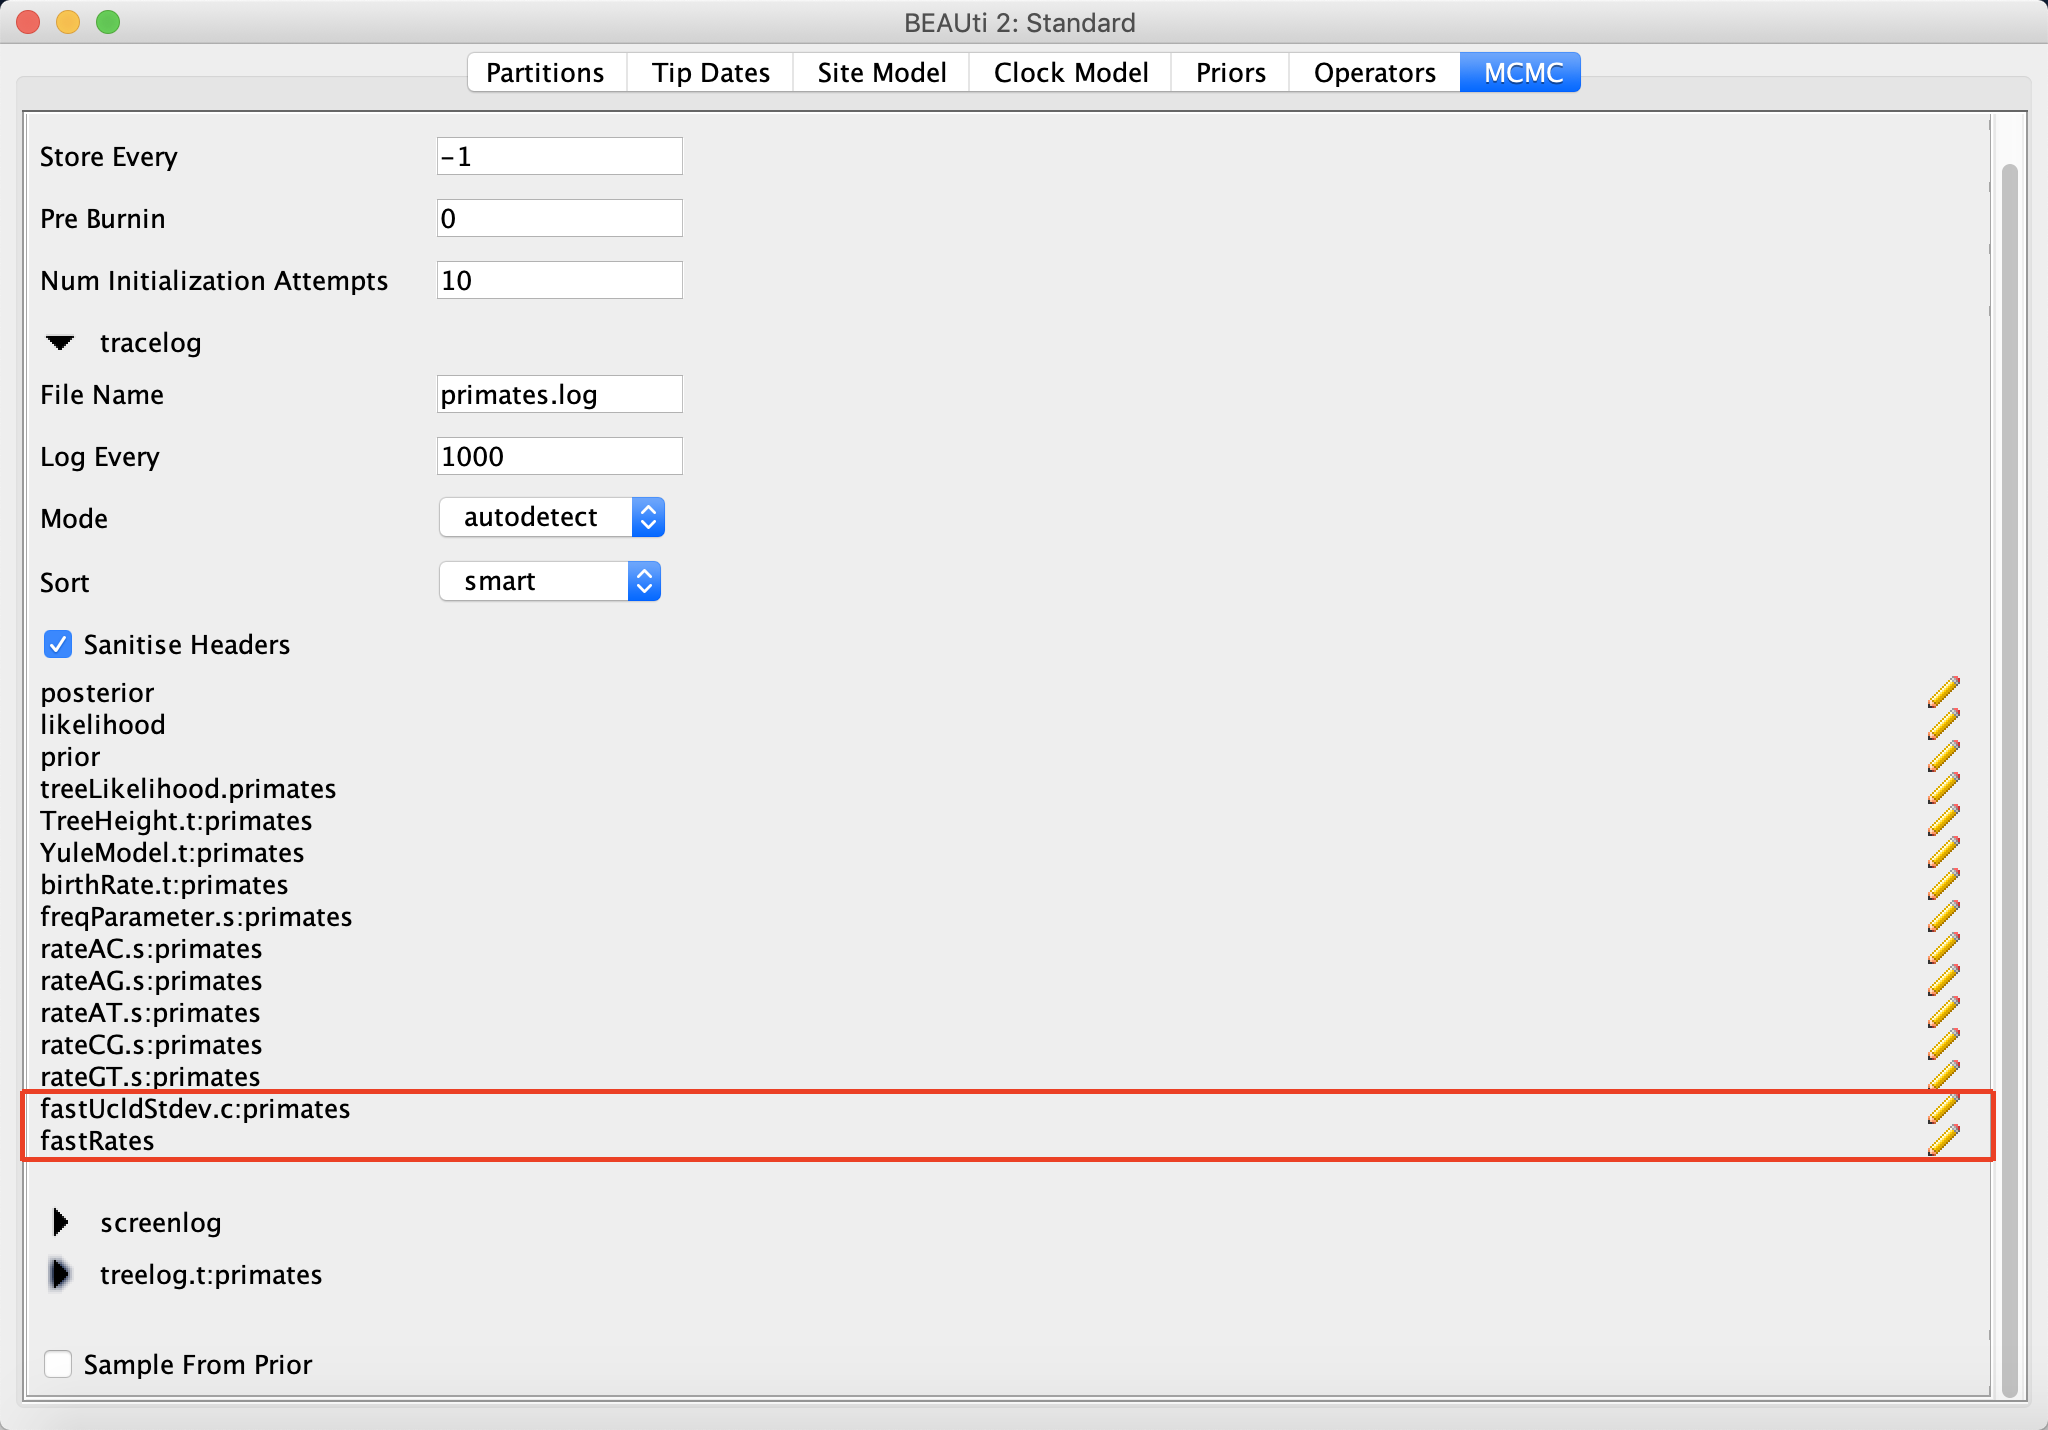
\includegraphics[width=0.750000\textwidth]{figures/trace_log.png}
\caption{specify trace logger}
\label{fig: trace-log}
\end{figure}

\item Save specifications

Finally, after all specifications are done (e.g., ``Partitions", ``Tip Dates", "Site Model"), you will need to save the configurations as .xml file by clicking on "File -> Save" and choosing the path (Fig.\ref{fig: save-xml}).
\begin{figure}
\centering
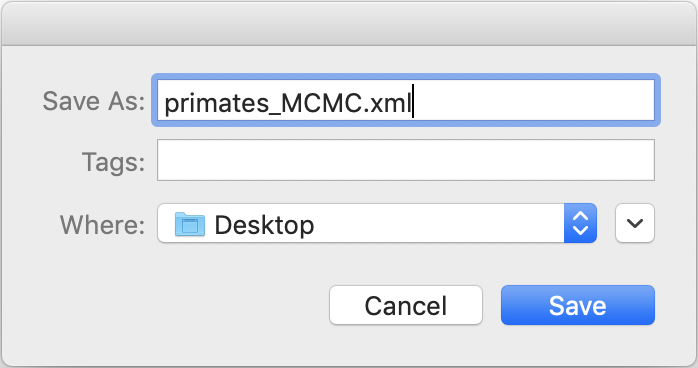
\includegraphics[width=0.500000\textwidth]{figures/save_xml.png}
\caption{save as .xml file}
\label{fig: save-xml}
\end{figure}

\end{enumerate}

\subsection{Run XML in BEAST2}
To run the analysis, you will need to specify main class as ``beast.app.beastapp.BeastMain" and use ``ConstantDistanceOperator" as module in configuration. Then, choose the previously generated .xml file, as is shown in Fig.\ref{fig: input-xml}.
\begin{figure}
\centering
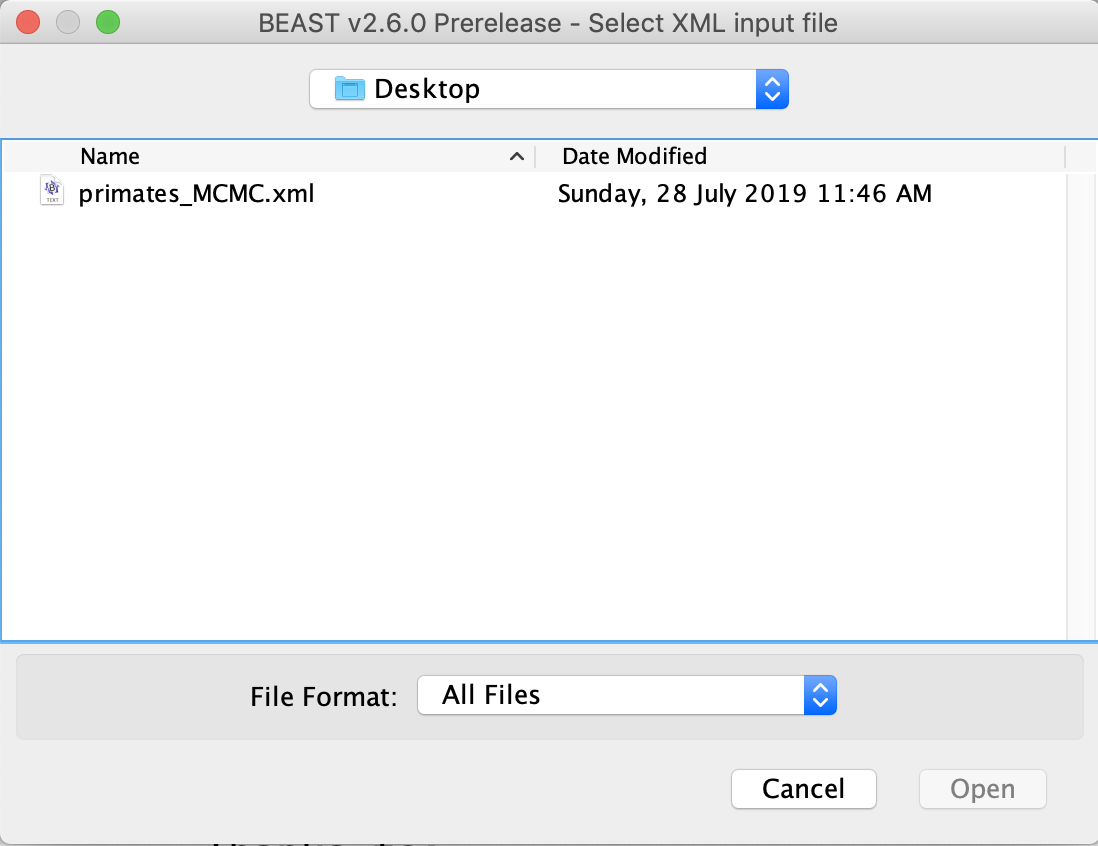
\includegraphics[width=0.500000\textwidth]{figures/input_xml.png}
\caption{input .xml file}
\label{fig: input-xml}
\end{figure}

\subsection{Analyse results}
After running BEAST2, three files are generated under the working directory, such as ``primates.log", ``primates.trees" and ``primates\_MCMC.xml.state". By loading .log file in Tracer and .trees file in FigTree, you are able to analyse the results. 

\section{Acknowledgment}\label{acknowledgment}

The content of this tutorial is based on the paper ``Improving the performance of Bayesian phylogenetic inference under relaxed clock models".

\section{Useful Links}\label{useful-links}
\begin{itemize}
\item
  \href{http://www.beast2.org/book.html}{Bayesian Evolutionary Analysis
  with BEAST 2} \citep{BEAST2book2014}
\item
  \href{https://github.com/denisekuehnert/bdmm}{Multi-type birth-death
  process package} \citep{Kuhnert2016}
\item
  BEAST 2 website and documentation: \url{http://www.beast2.org/}
\end{itemize}

%%%%%%%%%%%%%%%%%%%%%%%
% Tutorial disclaimer %
%%%%%%%%%%%%%%%%%%%%%%%
% Please do not change the license
% Add the author names and relevant links
% Add any other aknowledgments here
\href{http://creativecommons.org/licenses/by/4.0/}{
\includegraphics[scale=0.8]{figures/ccby.pdf}} This tutorial was written by Rong Zhang and Alexei Drummond for \href{https://taming-the-beast.github.io}{Taming the BEAST} and is licensed under a \href{http://creativecommons.org/licenses/by/4.0/}{Creative Commons Attribution 4.0 International License}. 

%%%%%%%%%%%%%%%%%%%%
% Do NOT edit this %
%%%%%%%%%%%%%%%%%%%%
Version dated: \today



\newpage 
%%%%%%%%%%%%%%%%
%  REFERENCES  %
%%%%%%%%%%%%%%%%

\printbibliography[heading=relevref]


\end{document}
